%%%%%%%%%%%%%%%%%%%%%%%%%%%%%%%%%%%
%                 Wrocław, grudzień 2012r.
%    Pracownia z Analizy Numerycznej M
%      Sprawozdanie z zadania p2.2
%         Łukasz Czapliński
%%%%%%%%%%%%%%%%%%%%%%%%%%%%%%%%%%%
\documentclass[11pt,wide]{mwart}

\usepackage[utf8]{inputenc} 
\usepackage[OT4,plmath]{polski}
\usepackage{graphicx}      
\usepackage{caption}
\usepackage{subcaption}
\usepackage{longtable}
\usepackage{amsmath,amssymb,amsfonts,amsthm,mathtools}

\usepackage{bbm}           
\usepackage[colorlinks=true]{hyperref}
                          
\usepackage{url}
%%%%%%%%%%%%%%%%%%%%%%%%%%%%%%%%%5
\title{{\textbf{Pracownia z analizy numerycznej\\}}
       {\Large Sprawozdanie do zadania \textbf{P2.2}\\}
       {\large Prowadzący: dr Paweł Woźny}}
\author{Łukasz Czapliński\\  e-mail: \texttt{czapl.luk@gmail.com}}
\date{Wrocław, dnia \today\ r.}

\begin{document}
\thispagestyle{empty}
\maketitle
\newpage
\section{Wstęp}
\subsection{Słowo wstępu}
Numeryczne szukanie miejsca zerowego funkcji to temat wyjątkowo obszerny. Paradoksalnie może się jednak wydawać że wszystko zostało już w tym temacie omówione i zbadane. Znane są metody pozwalające bardzo szybko zwiększać dokładność, z jaką szacujemy miejsce zerowe (jak metoda Newtona), jak i pozwalające określać dobrze te początkowe przybliżenia (jak metoda bisekcji). Łącząc kilka takich metod otrzymujemy narzędzie, wydawać by się mogło, idealne. Dobrym przykładem jest tu metoda Brenta. Jednak takie konglomeraty, rozważające w każdym kroku, której ze swoich podmetod użyć mają zadaniczą wadę: procesor wykonuje je wolniej. O wiele szybciej liczone są te, które w każdym kroku pętli po prostu wyliczają kolejne przybliżenie i sprawdzają czy jest ono dość dokładne, zamiast najpierw wykonywać kilka "if'ów". W tej pracowni omówie 3 takie metody: dobrze znane metody stycznych i siecznych oraz mniej znaną odwrotnej interpolacji kwadratowej.
\subsection{Opis metod}
Praktycznie każdy, kto choć chwilę interesował się tematem analizy numerycznej zna metody siecznych i stycznych.\\
\indent Metoda siecznych liczy kolejne przybliżenia ze wzoru:
\begin{gather}
  x_{n+1} = x_{n} - \frac{y_{n}*(x_{n} - x_{n-1})}{y_{n} - y_{n-1}}
\end{gather}
\indent Z kolei metoda stycznych ze wzoru:
\begin{gather}
  x_{n+1} = x_{n} - \frac{y_{n}}{y'_{n}}
\end{gather}
\indent Intuicyjnie oznacza to tyle, że przybliżamy funkcję $y=f(x)$ w otoczeniu $x_{n}$ przez funkcję liniową (metoda siecznych wykorzystuje w tym celu 2 poprzednie wartości $x$, a metoda stycznych pochodną funkcji $f$), a następnie za kolejne przybliżenie $x_{n+1}$ przyjmujemy miejsce zerowe tej funkcji liniowej. Poprzez analizę tych wzorów można też wykazać, że rząd zbieżnosci metody stycznych jest większy niż rząd zbieżnosci metody siecznych (rząd zbieżności określa jak bardzo kolejne zastosowanie metody zwiększy precyzję wyznaczonego przybliżenia miejsca zerwego).\\
\indent Trzecia metoda, odwrotnej interpolacji kwadratowej, ma trochę bardziej zawiły wzór:
\begin{gather}
  x_{n+1} = \frac{x_{n-2}*y_{n-1}*y_{n}}{((y_{n-2}-y_{n-1})*(y_{n-2}-y_{n}))} + \frac{x_{n-1}*y_{n-2}*y_{n}}{((y_{n-1}-y_{n-2})*(y_{n-1}-y_{n}))} + \frac{x_{n}*y_{n-2}*y_{n-1}}{((y_{n}-y_{n-2})*(y_{n}-y_{n-2}))}
\end{gather}
\indent Odpowiada to przybliżeniu danej funkcji $y=f(x)$ przez funkcję kwadratową, wykorzystując 3 poprzednie wartości $x$, a następnie znalezieniu jej miejsca zerowego przez wyliczenie funkcji do niej odwrotnej $g = f^{-1}$ i wartości $g(0)$ (ponieważ $g = f^{-1} \Rightarrow x_0 = g(0) \Leftrightarrow f(x_0) = 0)$. Tutaj już pojawia się pierwsza wątpliwość: przecież nie zawsze istnieje funkcja odwrotna do funkcji kwadratowej na zadanym przedziale, co wtedy? Kolejnym pytaniem jest: jeśli ta metoda działa, to jaki jest jej rząd zbieżności? Czy jest porównywalna z którą z poprzednich metod?
\subsection{O programie}
Aby rzetelnie odpowiedzieć na te pytania, napisany został obszerny program testujący. Składa się on z kilku modułów.
Pierwszy z nich odpowiada za parsowanie i obliczanie wartości funkcji. 
Znajduje się w pliku fhb.cpp.
Pozwala na stworzenie struktury \begin{verbatim}fhb::fun_wrap\end{verbatim} za pomocą konstruktora \begin{verbatim}fhb::fun_wrap(string s)\end{verbatim} gdzie s zawiera wzór funkcji - więcej o nim dalej - i liczenie wartości tej funkcji w punkcie x za pomocą metody \begin{verbatim}double fhb::fun_wrap::apply(double x)\end{verbatim}
Kolejny, zawarty już w program.cpp odpowiada za implementację omawianych metod.
Aby wymusić możliwie najlepsze warunki do porównania czasu działania metod, zostały one napisane w stylu funkcyjnym: każda z funkcji implementujących metodę składa się z procedury odpowiadającą za jeden krok obliczeń: mając daną funkcję i ciąg przybliżen, zwraca ona kolejne przybliżenie.
Nie ma tu spamiętywania: każda procedura wylicza wszystkie potrzebne wartości funkcji. Później wyjaśnię powód tak nieoptymalnego rozwiązania.
Funkcja ta jest następnie iterowana (przez funkcję iterate), aby uzyskać ciąg kolejnych przybliżen miejsca zerowego.\\
{\small{Nota o badaniu zbieżności w programie.\\ Warunki stopy zostały dobrane tak, żeby obliczenia zatrzymywały się, gdy obliczenia są zbieżne do jakiegokolwiek miejsca zerowego. Funkcja iterująca w żaden sposób nie bada odległości od przewidywanego przez nas miejsca zerwego.}}
\\Trzeci moduł to funkcja \begin{verbatim}do_computations\end{verbatim} która odpowiada za komunikację programu z użytkownikiem.
Przyjmuje jako argumenty metodę, jej nazwę oraz nazwę testu, który ma być wykonany, następnie wczytuje test z pliku \begin{verbatim}"./testy/<nazwa_testu>.din"\end{verbatim} i wypisuje kolejno wyniki:\\
\begin{tabular}{l l}
   \hline
  co?                                                       & gdzie? - nazwa pliku\\
  \hline
  ciąg przybliżen miejsca zerowego                          & 
    \begin{minipage}{3in} \begin{verbatim}"./wyniki/<nazwa_testu>/<nazwa_metody>.dw"\end{verbatim} 
      \end{minipage}\\
  rząd zbieżności dla kolejnych przybliżen                  & 
     \begin{minipage}{3in} \begin{verbatim}"./wyniki/<nazwa_testu>/<nazwa_metody>.dr"\end{verbatim} 
      \end{minipage}\\
  statystyki (czas, ilość iteracji, średni rząd zbieżności) & 
    \begin{minipage}{3in} \begin{verbatim}"./wyniki/<nazwa_testu>/<nazwa_metody>.dt"\end{verbatim} 
      \end{minipage}\\
\end{tabular}
\\ \\ \indent Ogólnie sam program przyjmuje jako argument nazwę testu i wywołuje 
\begin{verbatim}do_computations\end{verbatim} dla wszystkich 3 metod.
Dodatkowo zamieszczone zostały skrypty (w folderze "./skrypty"). Główny z nich - replot.sh - upewnia się, że istnieje odpowiednia struktura katalogów (tworzy wymagane, jeśli ich nie ma), kompiluje program, wywołuje go dla każdego testu z foldery "./testy", następnie tworzy plik z poleceniem dla gnuplota, wywołuje gnuplota by stworzył wykresy i umieszcza je w folderze "./wykresy". Następnie wywołuje pdftex'a, by ponownie stworzył sprawozdanie (ze zmienionymi wykresami) i usuwa zbędne pliki.
\subsubsection{O parserze}
Używany parser z pliku
\begin{verbatim}fhb.cpp\end{verbatim}
został napisany przez autora jako projekt na ANSI C zanim poznał on słowo "parser", więc naturalnie ma pewne ograniczenia:
\begin{enumerate}
\item
  Nie obsługuje on potęg. Tak więc $x^2$ należy podać jako $x*x$.
\item
  W funkcji może występować tylko jedna zmienna i należy ją oznaczyć jako $x$.
\item
  Niedozwolone są znaki białe - nie powinna wystąpić żadna spacja we wzorze funkcji.
\item
  Obsługiwane są tylko wbudowane funkcje: $sin$, $cos$, $sqrt$, $ln$ i specjalna $mpi$. Każda z nich musi otrzymać jakiś argument - funkcję w nawiasach $( )$ lub samo $x$. Funkcja $mpi$ zwraca zawsze PI, niezależnie od argumentu.
\item
  Poza tym argument - string może być dowolną (matematycznie poprawną) funkcją składającą się ze znaków: $x$, $*$, $/$, $+$, $-$, nawiasów $( )$ i stałych.
\end{enumerate}

\subsubsection{Struktura testu}
Test powinien się składać z .. linii. Powinny one wyglądać następująco:
\begin{enumerate}
  \item
    ciąg znaków - 3 liczby typu double (w notacji angielskiej, $.$ zamiast $,$) - kolejne przybliżenia miejsca zerwego. W kolejności od najmniej dokładnego do najbardziej. Oddzielone spacjami.
  \item
    ciąg znaków - funkcja, której miejsce zerowe szukamy. Format taki, jak dla parsera.
  \item
    ciąg znaków - pochodna powyższej funkcji. Format jw.
  \item
    ciąg znaków - funkcja 0-argumentowa w formacie dla parsera - dokładne miejsce zerowe funkcji. Pozwala to wygodnie podawać miejsca zerowe funkcji trygonometrycznych. Program sprawdza po wczytaniu czy faktycznie funkcja ta daje stałą wartość dla różnych wyrażeń.
\end{enumerate}
\section{Wyniki doświadczenia}
\subsection{Ogólne spojrzenie na wyniki}
Oto pełne wyniki przeprowadzonych doświadczeń.
\begin{table}[h]
  \begin{tabular}{| l l | l l l|}
  \hline
  n & Funkcja & \multicolumn{3}{|c|}{Przybliżenia}\\
  \hline 
test0
&
x*x-9
&
0
&
1.5
&
2.5
\\
test1
&
x*x+x-6
&
0.
&
-1.5
&
-2.
\\
test2
&
sin(x)+1
&
0.
&
-1.
&
-1.5
\\
test3
&
x+sin(x-3)-3
&
1.
&
1.8
&
2.7
\\
test4
&
-x*x+4
&
1.
&
-1.
&
-1.5
\\
test5
&
-x*x+9
&
2.
&
1.
&
0.
\\
test6
&
sin(x)*(x+1)
&
1.
&
0.7
&
0.5
\\
test7
&
x*x*x*x-16
&
1.5
&
1
&
-1
\\
\hline
\end{tabular}\\\\
\begin{tabular}{| l | l l l l| l l l l| l l l l|}
\hline
 & \multicolumn{4}{|c|}{met sty} & \multicolumn{4}{|c}{met siecz} & \multicolumn{4}{|c|}{odwr interpol kw}\\
\hline 
 n &
 t & i & r & m &
 t & i & r & m &
 t & i & r & m \\
\hline

test0
&
24
&
8
&
1.99
&
3
&
66
&
10
&
1.82
&
3
&
41
&
10
&
1.93
&
3
\\
test1
&
36
&
9
&
1.99
&
-3
&
83
&
11
&
1.63
&
-3
&
55
&
11
&
1.98
&
-3
\\
test2
&
98
&
27
&
0.482
&
-1.57
&
306
&
103
&
0
&
-nan
&
174
&
33
&
0.621
&
-1.57
\\
test3
&
56
&
7
&
2.51
&
3
&
96
&
8
&
2.17
&
3
&
55
&
9
&
1.84
&
3
\\
test4
&
23
&
8
&
2.04
&
-2
&
67
&
10
&
1.72
&
-2
&
310
&
103
&
0
&
nan
\\
test5
&
313
&
103
&
0
&
-nan
&
75
&
14
&
-0.00856
&
3
&
26
&
5
&
1.76
&
-3
\\
test6
&
78
&
9
&
1.98
&
0
&
86
&
11
&
1.62
&
3.26e-28
&
64
&
10
&
1.85
&
3.85e-34
\\
test7
&
52
&
13
&
2
&
-2
&
426
&
103
&
0
&
-nan
&
474
&
103
&
0
&
-nan
\\
    \hline  
  \end{tabular}\\\\
  \begin{tabular}{r | l}
    Przybliżenia  & Szacunkowe wartości miejsca zerowego, od których zaczynać miały metody\\
    t             & Czas wykonywania obliczeń w mikrosekundach\\
    i             & Ilość wykonanych iteracji \\ & \indent (wartość 103 oznacza, że nie udało się znaleźć dość dobrego przybliżenia)\\
    r             & Średnia wartość numerycznego rzędu zbieżności\\
    m             & Ostatnie przybliżenie miejsca zerowego\\
  \end{tabular}
\end{table}

\\\indent Patrząc ogólnie na powyższe wyniki można zauważyć, że metoda stycznych w większości przypadków jest o wiele lepsza od metody stycznych czy też odwrotnej interpolacji kwadratowej. Potwierdza to spojrzenie na wykresy \ref{fig:test4} i \ref{fig:test0}.
\begin{figure}[ht]
  \begin{minipage}[b]{0.45\linewidth}
    \centering
    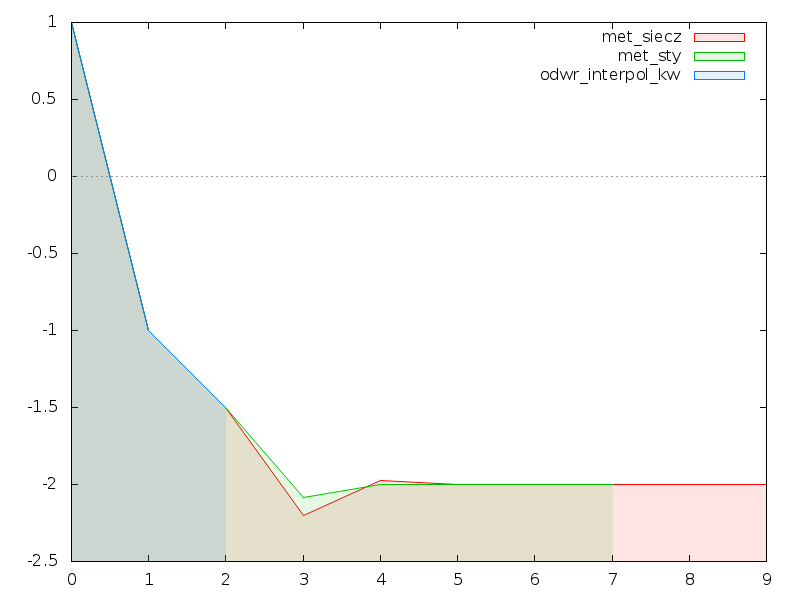
\includegraphics[width=\textwidth]{../wykresy/test4.png}
    \caption{Ilość cyfr dokładnych n-tego przybliżenia dla test4.din}
    \label{fig:test4}
  \end{minipage}
  \hspace{0.5cm}
  \begin{minipage}[b]{0.45\linewidth}
    \centering
    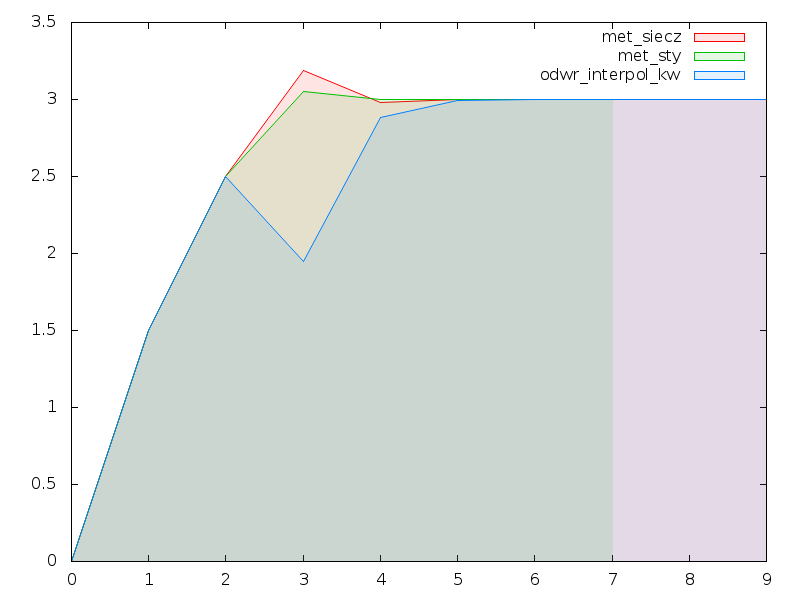
\includegraphics[width=\textwidth]{../wykresy/test0.png}
    \caption{Ilość cyfr dokładnych n-tego przybliżenia dla test0.din}
    \label{fig:test0}
  \end{minipage}
\end{figure}
\\ \indent Ciekawsze jednak wydają się te przypadki, w których któraś z metod okazała się zbyt wolno zbieżna (test2, test4, test5, test6, test7). Przyjrzyjmy się im dokładniej.
{\small{\\Wykresy można znaleźć w katalogu "./wykresy". Dla każdego testu znajduje się tam wykres $y = x_{n}$, rzędu zbieżności oraz wartości, które znajdują się w tabelce powyżej. Z kolei numeryczne wartości są w plikach wymienionych przy opisie programu. }} 
\subsection{Brak zbieżności metod}
Widzimy, że każda z metod dla pewnych warunków startowych nie jest zbieżna do miejsca zerowego (czasem, jak w teście 5 bywa zbieżna do innego miejsca zerowego). Metoda siecznych nie jest zbieżna, gdy prosta przechodząca przez punkty $(x_{n}, f(x_{n}))$ i $(x_{n+1}, f(x_{n+1}))$ jest równoległa do ox. Metoda stycznych - gdy $f'(x_{n}) = 0$. Z kolei odwrotna interpolacja kwadratowa - gdy nie ma funkcji odwrotnej $g = y^{-1}$ na zadanym przedziale (gdzie $y \in \Pi_2$ interpoluje $f$ w $x_{n}$, $x_{n-1}$, $x_{n-2}$).
Widać tu podobieństwo metody siecznych i odwrotnej interpolacji kwadratowej - obie mają duże problemy z funkcjami, które nie są rożnowartościowe w zadanym otoczeniu miejsca zerowego. Mogłoby się wydawać, że odwrotna interpolacja kwadratowa, dzięki temu, że bierze więcej punktów powinna być bardziej odporna na perfidny ich wybór. Jak się okazuje, tak nie jest: była ona zawodna w większości przypadków, w których zawodziła metoda siecznych, a także w innych. Metoda stycznych przeszła wszystkie testy, które nie były specjalnie w nią wymierzone. Na korzyść odwrotnej interpolacji kwadratowej przemawia fakt, że jej rząd zbieżności był lepszy niż metody siecznych. Z tego powodu jej wykonanie było zwykle około 2-3x szybsze niż metody siecznych.
\section{Zakończenie}
Podsumowując, metoda odwrotnej interpolacji kwadratowej jest przydatna, gdy z jakichś powodów nie możemy zastosować metody stycznych (np nie znamy lub nie możemy policzyć pochodnej funkcji). Jest ona szybciej zbieżna niż metoda siecznych, lecz bardziej kapryśna niż metoda stycznych. Nawet bez spamiętywania jej wykonanie jest szybsze niż metody siecznych. Zastanawiające jest więc, czy metoda odwrotnej interpolacji sześciennej nie okazałaby się jeszcze lepsza, dodatkowo będąc pozbawioną wady braku funkcji odwrotnej w liczbach rzeczywistych. Problemem mogłoby być liczenie współczynników, lecz to temat na inną pracownię.
\end{document}

